\inputencoding{utf8}
\chapter[Testiranje zmogljivosti Amazon EC2 platforme (P. Matičič, J. Pelicon, B. Rojc)]{Testiranje zmogljivosti Amazon EC2 platforme}

\pagestyle{fancy}
\fancyhf{}
\fancyhead[LE,RO]{\thepage}
\fancyhead[RE,LO]{\leftmark}

\huge Peter Matičič, Jan Pelicon, Blaž Rojc
\normalsize
\bigskip

\section{Opis problema}

Z dneva v dan proizvedemo čedalje več slik.
Predstavljajo znaten delež podatkov, shranjenih v raznih storitvah v oblaku.
Ampak ko želimo najti določen predmet ali osebo, ki smo jo slikali, je ročno brskanje po digitalnih zbirkah zamudno.

S tem problemom v mislih bomo stestirali oblačno platformo Amazon EC2.
Ustvarili bomo enostavno storitev, ki bo uporabniku omogočala iskanje vzorcev v večjem naboru slik, shranjenih v oblaku.
Poglobili se bomo v zahtevnost uporabe za programerja, fleksibilnost pri programiranju in morebitnem prenašanju storitve na druge platforme,
	odzivnost in izkušnjo za uporabnika ter zmogljivost in skalabilnost virov na platformi.
	
	\begin{figure}[H]
    \centering
    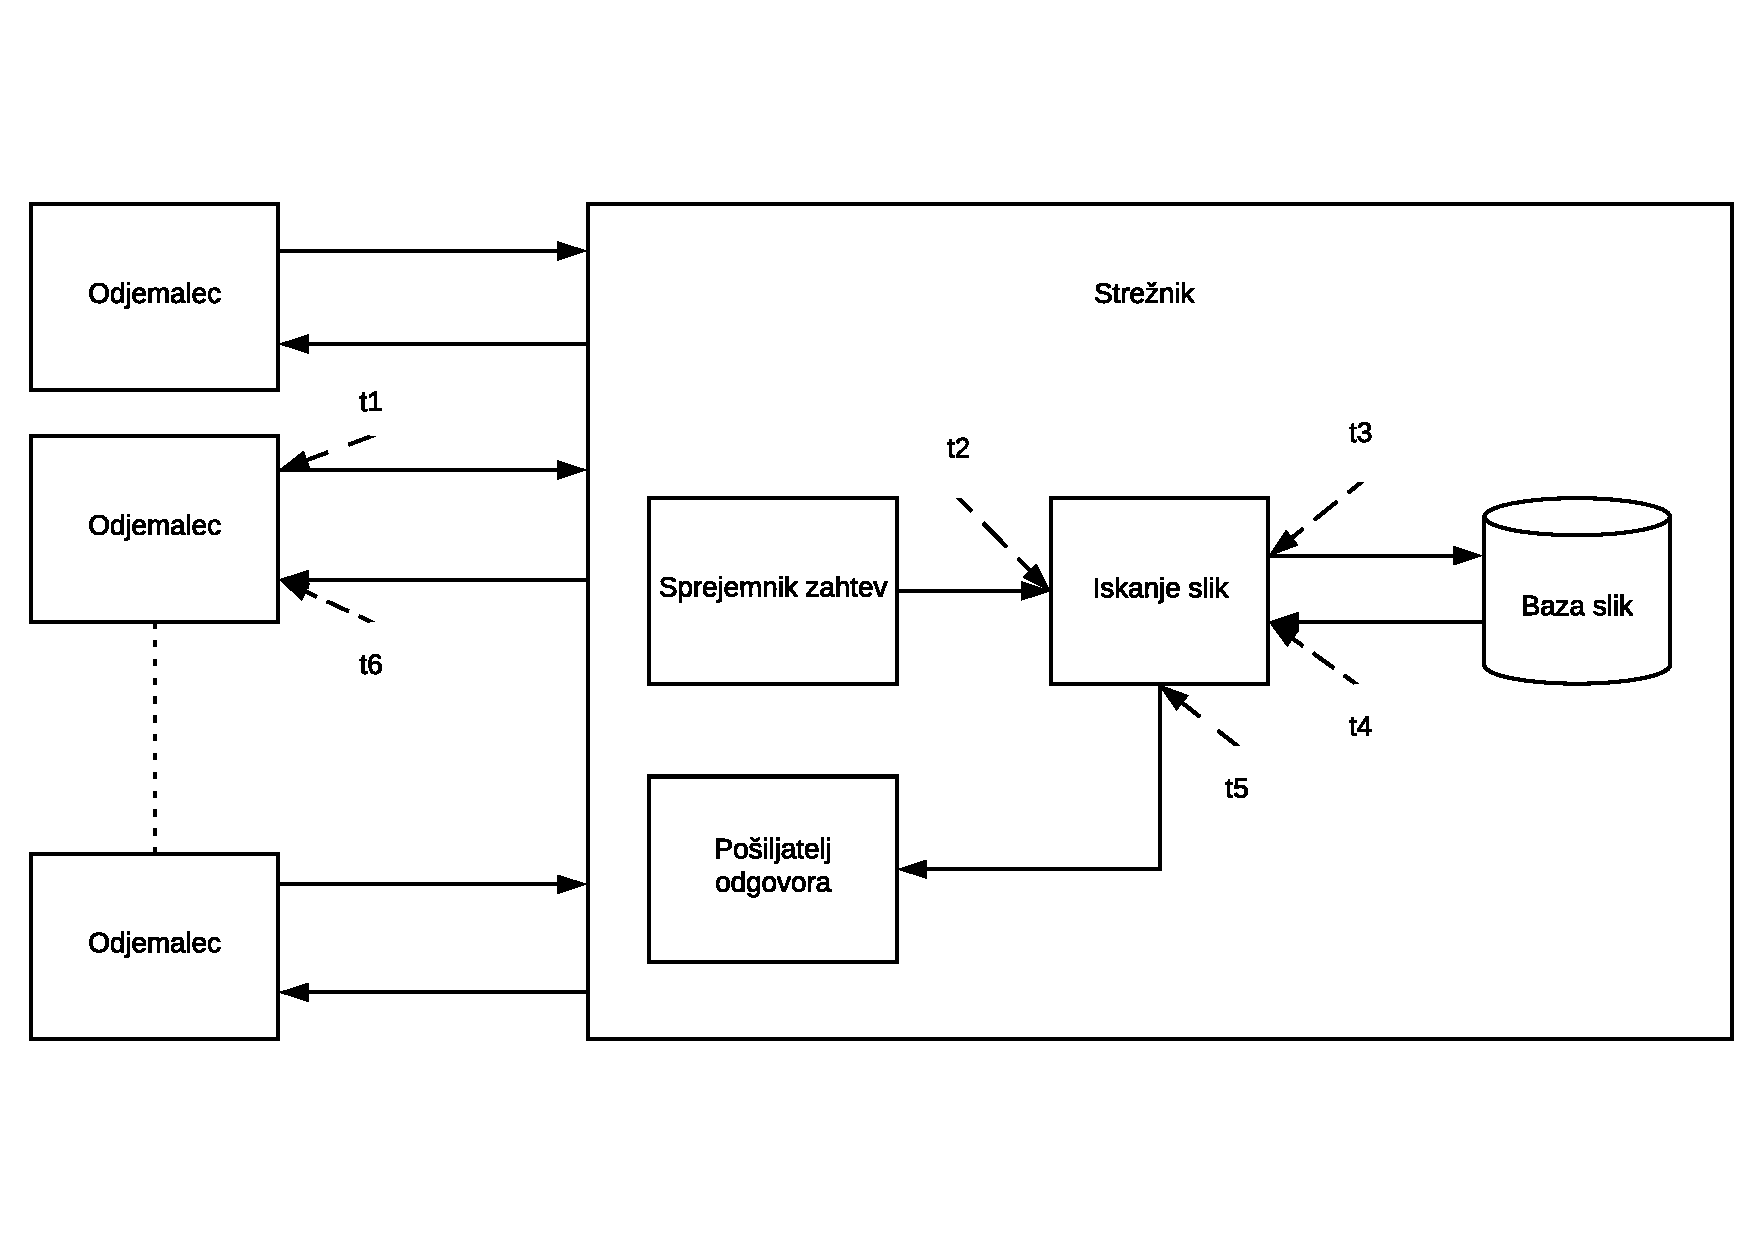
\includegraphics[scale=0.4]{Img/1_shema.pdf}
    \caption{Shema aplikacije.}
    \label{fig:1_osnovnaShema}
\end{figure}

\section{Realizacija}

\subsection{Način iskanja vzorca}
\begin{itemize}
\item Iskanje ene slikovne točke v množici slik ki bo ustrezala zahtevam.
\item Iskanje vzorca podanega z masko v mnžici slik.
\item Iskanje slike, ki vsebuje podan slikovni izsek.
\end{itemize}

\subsection{Amazon Web Services (AWS)}
Za delo z Amazon Web Services si mora uporabnik ustvariti račun v njihovem sistemu. Po uspešni registraciji si lahko ustvarimo svojo instanco EC2 storitve, ki nam jo Amazon ponuja zastonj za eno leto pri čemer na mesec porabimo največ 750 ur delovanja. Obsežnejša navodila so navoljo tudi na Amaznovi spletni strani \cite{1_aws_ec2_tutorial}, mi pa smo to naredili tako, da se postavimo v AWS Management Console, kjer lahko izberemo opcijo Launc a virtual machine with EC2. Takoj nam konzola ponudi izbiro slike, katero bi uporabljali na novi virtualki kot prikazano na sliki \ref{fig:1_AWS_images}. Za naš projekt smo izbrali sliko Amazon Linux 2 AMI c. 
\begin{figure}[H]
    \centering
    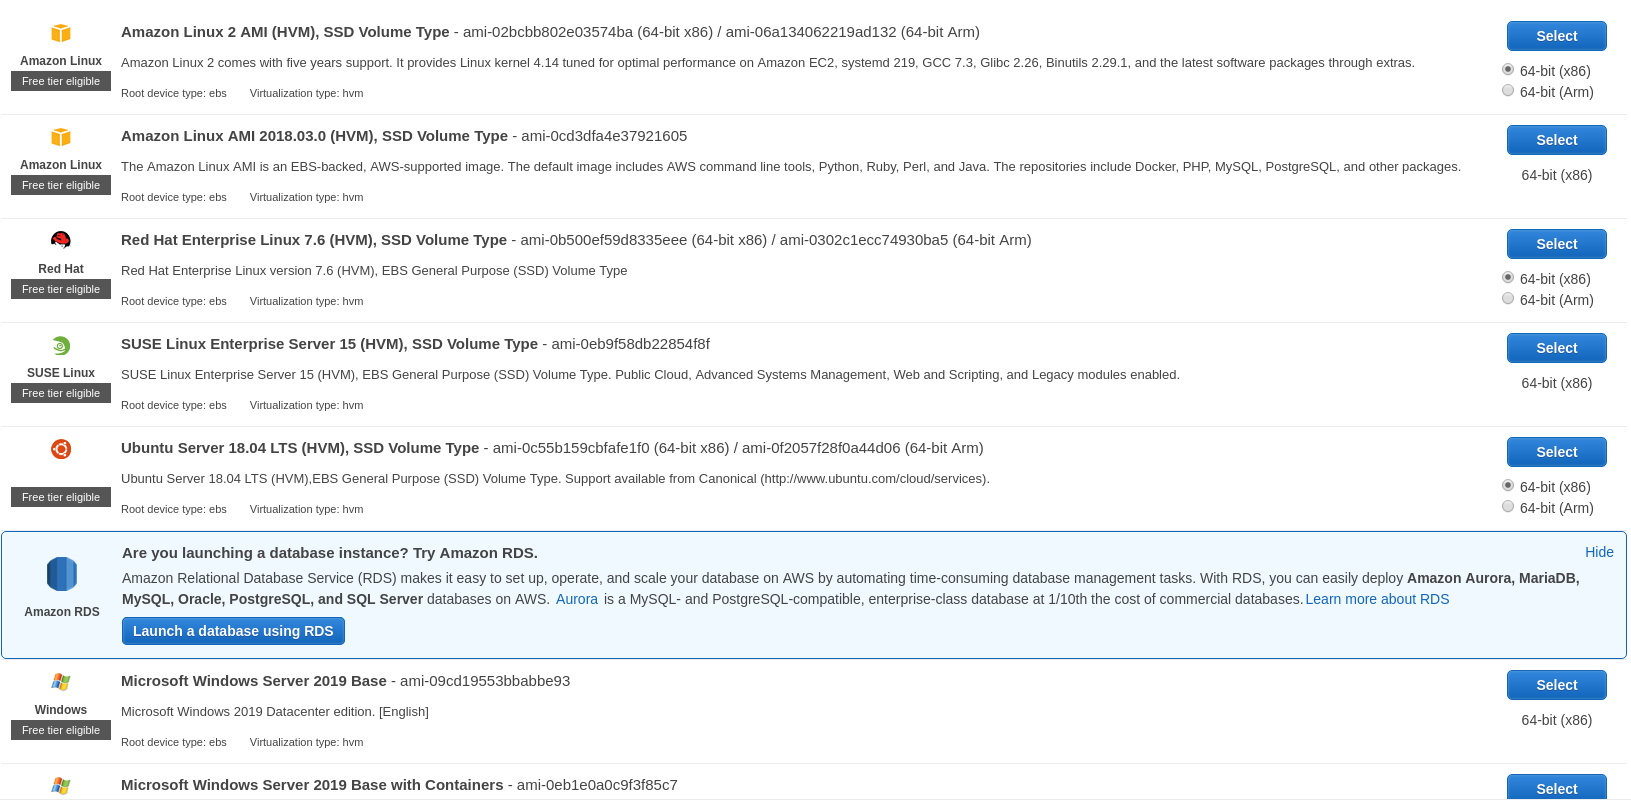
\includegraphics[scale=0.25]{Img/1_AWS_images.png}
    \caption{Slike za izdelavo virtualke}
    \label{fig:1_AWS_images}
\end{figure}
V naslednjem koraku izberemo tip instance slike, to je Amazonov način izbire paketov, ki vključujejo različne funkcionalnosti. V našem primeru ker izbiramo zastonjsko različico nam ponujajo tip t2.micro, ki vsebuje 1 jedro, 1GB pomnilnika, samo začasno hranjenje podatkov na disku in nižjo hitrost povezave. Za tem lahko nadaljujemo z nastavljanjem različnih konfiguracij naše virtualke ali pa preprosto kliknemo Review and Launch, ki nam ponudi še en pregled čez izbrane nastavitve in zažene virtualko.  Po zagonu virtualke nam sistem ponudi opcijo generiranja para ključev za varno SSH povezavo nanjo. Ko zaključimo z ustvarjanjem, se premaknemo v EC2 management console kjer kliknemo na instances in od tam lahko opazujemo status naše storitve in pridobimo tudi naslov na katerem se nahaja. Za povezavo uporabimo javni naslov storitve, uporabnika $ec2-suser$ za varnost pa uporabimo $.pem$ datoteko, ki smo jo v prejšnjem koraku prenesli. Ko se uspešno povežemo na storitev lahko pričnemo z razvojem naše aplikacije.

\subsection{Aplikacija}
Aplikacija je napisana v programskem jeziku Java. Sestavljata jo odjemalska in strežniška komponenta, ki uporabljata skupne enumeratorje za določanje tipa zahteve. Zahteve sestavlja odjemalec in jih pošlje strežniku, ki to zahtevo obdela - začne iskanje v slikah in pripravi prvi najden rezultat. Povezava med strežnikom in odjemalcem je trajna, dokler je eden od njiju ne prekine, kar nam omogoči, da pri meritvah ne upoštevamo časa vzpostavitve povezave. Podatki se prenašajo v obliki JSON, ki vsebuje sekvenčno številko zahteve, tip zahteve in morebitne dodatne podatke, ki so potrebni za obdelavo. Strežnik ob prejemu podatkov začne z delom na ustrezni zahtevi ter nato pošlje odgovor klientu z številko zahteve in rezultatom. Strežniški del je napisan tako, da lahko paralelno obdeluje več zahtev.

\section{Predvidevanje metrik}
Kot glavno metriko bomo opazovali skupni čas zahteve in odgovora. Podrobneje ga bomo razdelili na čas potovanja zahteve od nas do strežnika ($t_2 - t_1$), čas obdelave na strežniku ($t_3 - t_2$) in čas potovanja odgovora od strežnika do nas ($t_4 - t_3$) (časi označeni na sliki \ref{fig:1_osnovnaShema}.

\section{Rezultati meritev}

\section{Plan dela}
\begin{itemize}
\item implementacija iskalnih algoritmov (0 / 3 narejenih)
\item določitev bremen
\item določitev metrik
\item določitev orodij
\end{itemize}

\section{Literatura}

\inputencoding{cp1250}